\subsection*{Data Sets}
\label{subsec:data_sets}
% energy calculations data set
The data set used for energy calculation experiments consisted of large protein structures, containing neither DNA, RNA, or modified residues with molecular masses between 100 and 150 kDa. 
All samples had resolutions better than 2 angstroms. 
The data set was filtered at 30\% sequence identity, and from this, 20 structures were selected at random, though two were later excluded due to technical reasons.
% Larger structures were used to better illustrate the performance improvement using this method.

% side chain prediction data set
The structures used in side chain prediction experiments consisted of high resolution enzyme structures.
Structures without an enzyme classification were excluded, as were structures with X-ray resolution less than 1.5 angstroms, or those with modified protein residues.
This resolution requirement was imposed to make high resolution side chain prediction comparisons more meaningful.
All structures had a molecular mass between 11 kDa and 110 kDa.
Structures containing DNA, RNA or modified side chain residues were excluded, as were those that had unreasonable steric clashes either within the canonical structure or with crystal neighbors.
Structures containing certain small molecules without energy parameterizations currently defined within PLOP were also excluded.

% structure preparation
\subsection*{Structure Preparation}
\label{subsec:structure_preparation}
In preparing the crystal structures for energy calculation and side chain prediction experiments, the first step was to add the crystal copies of the protein of interest.
PLOP completes this step for all space groups according to the crystal symmetry identified in the PDB file.
Before modeling a structure using an all atom force field, it is also necessary to add hydrogens and any missing heavy atoms.
When possible, PLOP uses the positions of bonded heavy atoms to build missing atoms into the structure.
However, adding hydrogens, especially for titratable residues, is a more complicated problem.
To address this, PLOP uses the independent cluster decomposition algorithm (ICDA) to determine the protonation states of any titratable residues, as well as the positions of polar hydrogens\cite{li2007assignment}.
Generally speaking, this proceeds by dividing titratable and polar residues into independent groups using a distance cutoff, and optimizing each group independently.
Structures with unreasonable steric clashes with crystal neighbors were removed from the data set on the basis that such structures are physically unlikely.

\subsection*{Grid-Based Spatial Indexing}
\label{subsec:grid_based_indexing}
Grid-based spatial indexing is a well known algorithm in computer science, especially computer graphics, that allows for efficient lookup based on geometric criteria and also provides fast collision detection\cite{bentley1979data}.
Critical to the present application, it allows constant time retrieval of a superset of atoms guaranteed to contain all atoms within a given euclidean distance.
%describe when/how you set the euclidean distance cutoff
In our implementation, the bounding box of the protein and its symmetric copies is subdivided along each of the orthogonal axes to form grid boxes or cells.
A simple convention for handling atoms that are positioned along cell boundaries guarantees that each atom is hashed to a unique cell.
For a single dimension, $d$, the cell index, or hash, of a point $p$ is 
\begin{equation}
i_{d}(p) = int\left(N * \frac{p_{d} - min_{d}(P)}{max_{d}(P) - min_{d}(P)}\right)
\end{equation}

where $min_d(P)$ and $max_d(P)$ are the minimum and maximum coordinates in dimension $d$ over the set of points $P$, $N$ is the number of cells in dimension $d$ and $p_{d}$ is the coordinate of $p$ in $d$.
Following the same procedure in each dimension gives a unique cell location for every atom.
In this way, at the beginning of the simulation, each atom is assigned to a specific cell, or grid box.
A list of the atoms in each grid box is then maintained over the course of the simulation.
When computing the electrostatic contribution to solvent free energy of an atom, $a$, it is only necessary to loop over the atoms contained in boxes that intersect the sphere corresponding to the distance cutoff around atom $a$. 
Beyond that cutoff, charge effects are considered to be negligible\cite{gallicchio2004agbnp}.

In the present implementation, cell size is at first set to 2.745 angstroms, and the number of cells in a given dimension depends on the "length" of the system in that dimension.
If the number of cells that this would require is unmanageably large, cells are then grown simultaneously in all dimensions such that the cell size is 1/250th of the longest dimension of the structure.

% cells figure, pretty
\begin{figure}[H]
\begin{center}
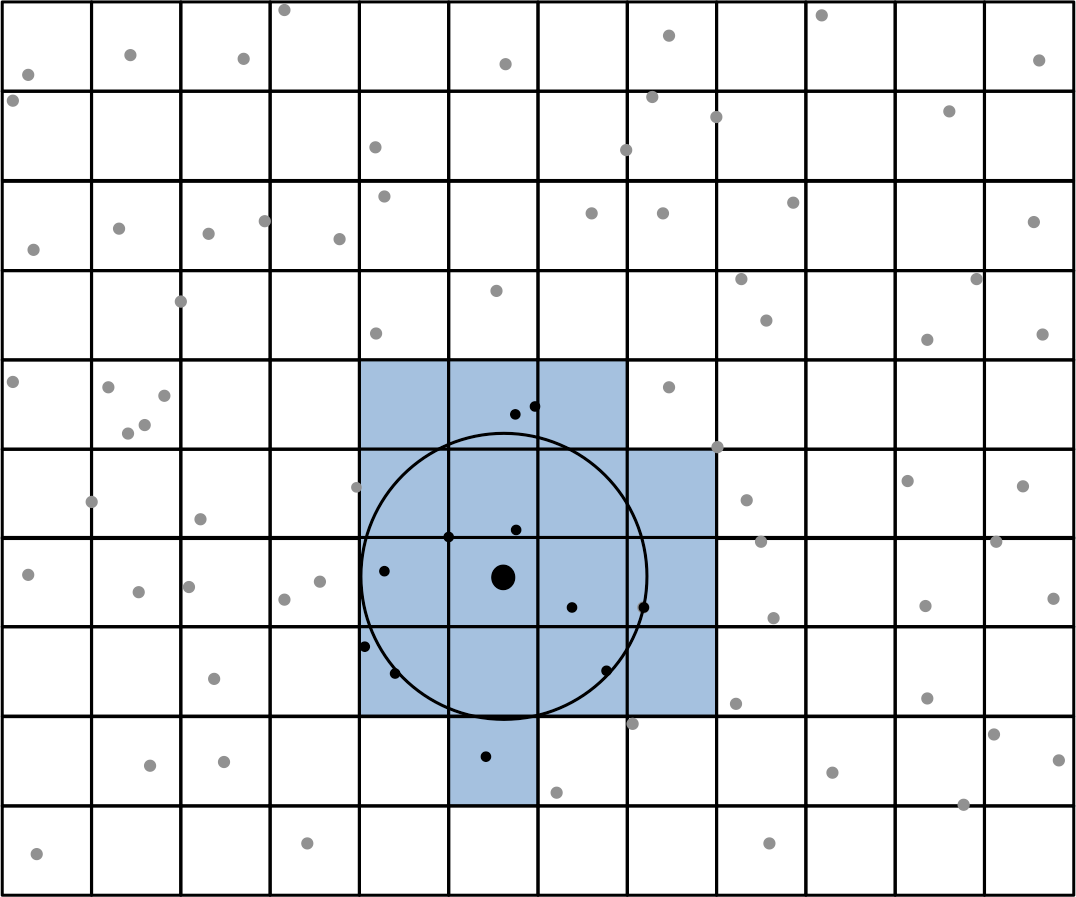
\includegraphics[width=3in]{figures/grid4_crop.png}
\caption{This illustrates, in two dimensions, the grid based spatial indexing method.
The naive S-GB method would require a distance computation to every other atom in the system.
By only considering atoms in cells intersecting the radius of influence, represented here in blue, it is possible to consider far fewer interactions.
Although only atoms inside the circle in this illustration contribute to surface charge, it is necessary to compute the distance over all black points.}
\label{fig:grid_hash}
\end{center}
\end{figure}

% side by side performance comparison figure
\begin{figure}[H]
\begin{center}
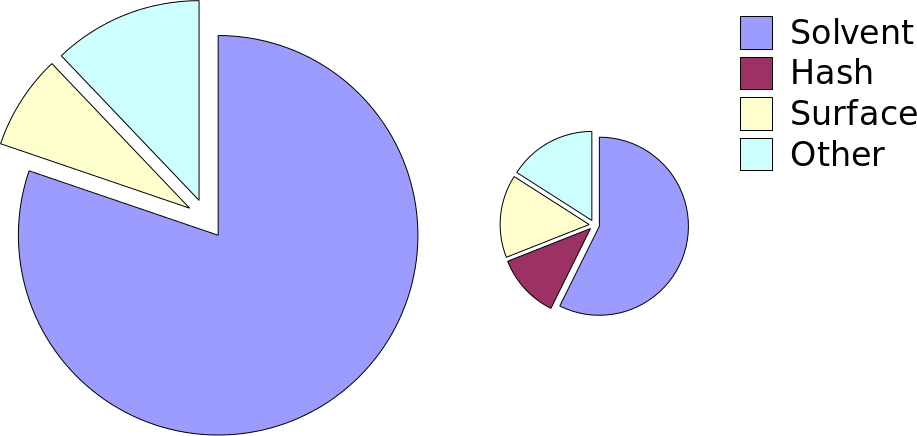
\includegraphics[width=3in]{figures/side_by_side.png}
\caption{Time spent during energy calculations on different parts of the energy model.
The left pie represents the non-cell based approach and the right pie the cell based approach, the charts are scaled relative the total cost of computing the energy.
One can see that although some overhead is introduced in maintaining the hash structure this significantly reduces the total cost of the solvent term, and as the solvent is such a large contributor to the total, also the total cost of computing the energy.}
\label{fig:timing_pie}
\end{center}
\end{figure}

\subsection*{Experiments}
\label{subsec:experiments}
% side chain prediction experiments
For side chain prediction, the specific side chains used were those which had at least 30\% solvent accessible surface area when evaluated in the absence of other chains or crystal neighbors.
Glycine and proline residues were also excluded, as they do not have free side chains.
Residues missing heavy atoms in the crystal structure were predicted; however, RMSD was not measured for these residues because there is no experimental data.
Side chain prediction experiments were performed as described in\cite{jacobson2002role}.

% energy calculations experiments
The experiment in this case consisted of multiple energy calculations, using the modified version of the OPLS-AA force field described in Li {\it et. al.} 2011\cite{li2011vsgb}.
In the control experiments, the same method for evaluating the implicit solvent term was used as in previous works.

